\documentclass{article}
\usepackage{polski}
\usepackage[utf8]{inputenc}
\usepackage{natbib}
\usepackage{graphicx}
\usepackage{xcolor}
\usepackage{mathtools}
\usepackage{amssymb}
\usepackage[makeroom]{cancel}
\usepackage{hyperref}
\newcommand{\norm}[1]{\left\lVert#1\right\rVert}

\title{Zadanie 16.12}
\author{Jan Bronicki}
\date{}


\begin{document}

\maketitle


Zakład Cehmiczny potrzebuje $10^{6}$ litra na dzień pewnej substancji. Trzy źródła są dostępne, mają różne ceny, dostęp oraz koncentracje nieczystości, gdzie nieczyzstości, gdzie nieczystości muszą byc poniżej pewnego poziomu.


\begin{figure}[h!]
    \centering
    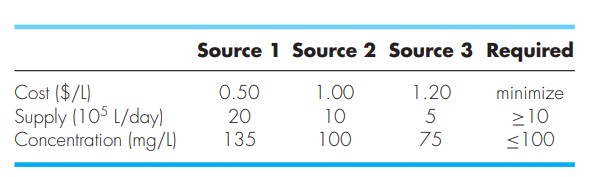
\includegraphics[scale=0.75]{sources.jpg}
\end{figure}


Musimy dobrać ilościowo różne źródła tak aby było to najoptymalniejsze kosztowo.

Niech $x_{1}, x_{2}, x_{3}$ oznaczają wartości (w L) ze źródeł 1, 2 i 3. Całkowity koszt kupna substancji:

$$
    f(x_{1}, x_{2}, x_{3})=0.5x_{1} + x_{2} + 1.2x_{3}
$$

Ponieważ $10^{6}$ litra jest potrzebne $x_{1} + x_{2} + x_{3} \geq 10^{6}$. Źródła też mają limity dlatego:

$$
    x_{1} \leq 2\cdot 10^{6}, \ x_{2} \leq 10^{6}, \ x_{3} \leq 5\cdot 10^{5}
$$

Aby utrzymać nieczystości poniżej ponadego poziomu:

$$
    135x_{1}+100x_{2}+75x_{3} \leq 100(x_{1}+x_{2}+x_{3})
$$


Przenosimy wszystkie wartości do Excela:


\end{document}